\documentclass[anchorcolor=blue,linkcolor=blue]{beamer}
\usepackage{booktabs}
\usepackage{amsmath}
\usepackage{xcolor}

\newcommand{\argmax}{\operatornamewithlimits{argmax}}
\newcommand{\rank}{\operatornamewithlimits{rank}}

\definecolor{links}{HTML}{07568E}
\hypersetup{colorlinks,linkcolor=,urlcolor=links}

%%\usepackage{blkarray}
\mode<presentation>
{
%  \usetheme{Malmoe}
\usetheme{default}
%\usecolortheme{seahorse}
  % or ...

 \setbeamercovered{transparent}
  % or whatever (possibly just delete it)
 \setbeamertemplate{footline}[default]
 \setbeamertemplate{navigation symbols}{\insertslidenavigationsymbol\insertframenavigationsymbol\insertdocnavigationsymbol}
}
\usepackage[english]{babel}

\title{\huge What can your library do for you?}
\author{Rajarshi Guha, Dac-Trung Nguyen,\\Alexey Zhakarov, Ajit
  Jadhav\\
\vskip 0.5em
NIH NCATS\\ \vskip 2em \textit{ACS Fall Meeting 2016, Philadelphia}}

\begin{document}

\begin{frame}
  \titlepage
\end{frame}

\begin{frame}
  \frametitle{Library Design}
  \begin{itemize}
  \item Historical collections and assay data provide information on how a set of compounds has faired
  \item Use (dis)similarity and machine learning to construct new collections that show similar behavior
    \begin{itemize}
    \item Plus various constraints
    \end{itemize}
  \item Libraries can be designed for certain target families or
    specific screening paradigms
  \item If sufficiently annotated, compound behavior can be correlated to assay and biology characteristics
  \end{itemize}
\end{frame}

\begin{frame}
  \frametitle{Two Questions}
  How likely are compounds, associated with a  given annotation, identified as active?
  \vskip 2em
  Given a new set of compounds, what sets of assay conditions (as implied by the annotations) will they be active in? 
\end{frame}

\begin{frame}
  \frametitle{BAO 2.0}
  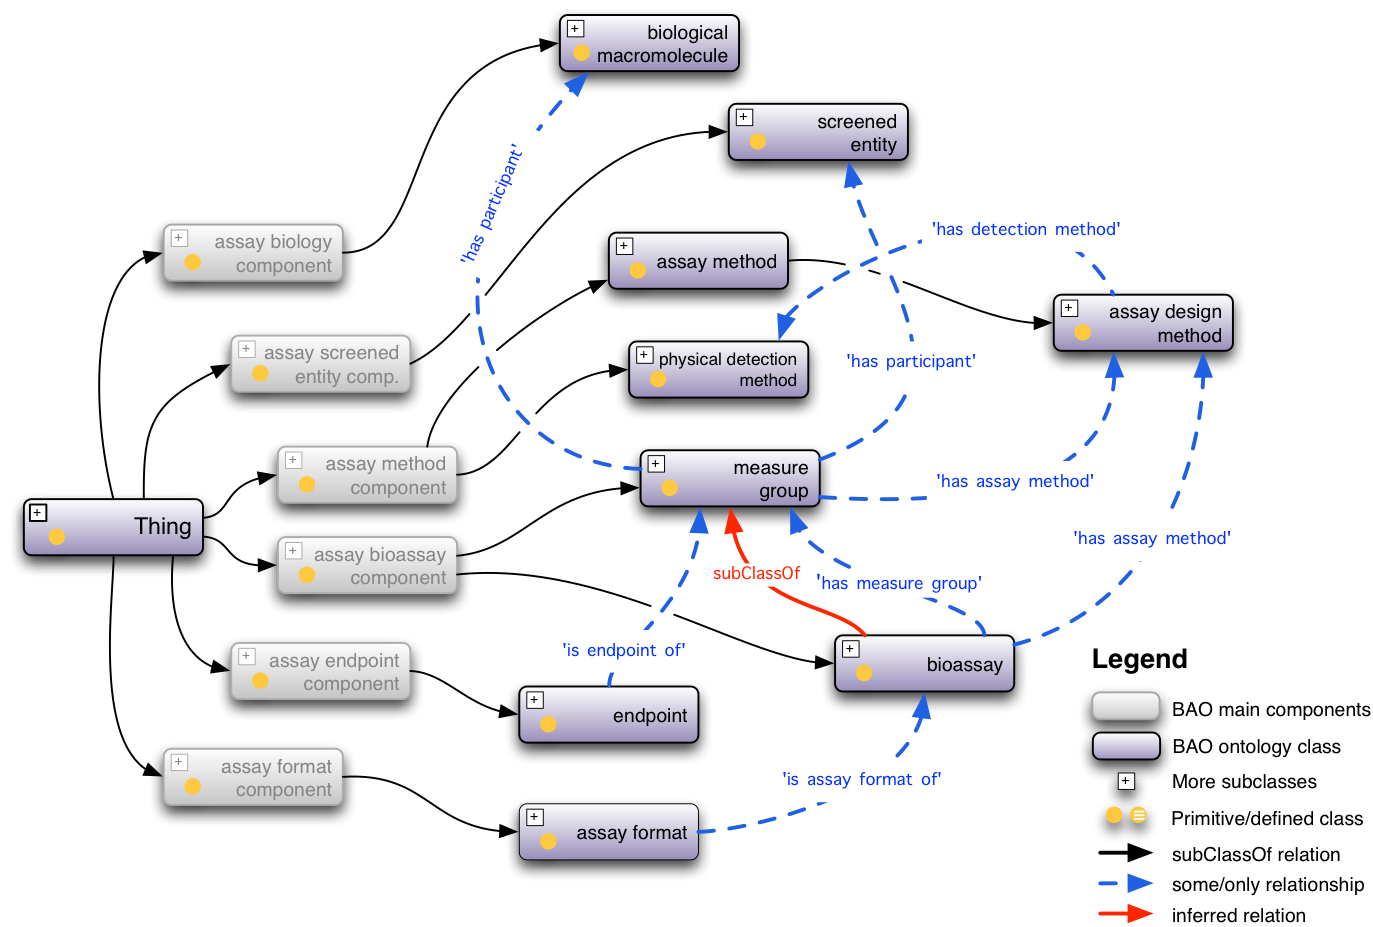
\includegraphics[height=3.0in]{bao}
\end{frame}

\begin{frame}
  \frametitle{Assay Modeling}
  \begin{center}
    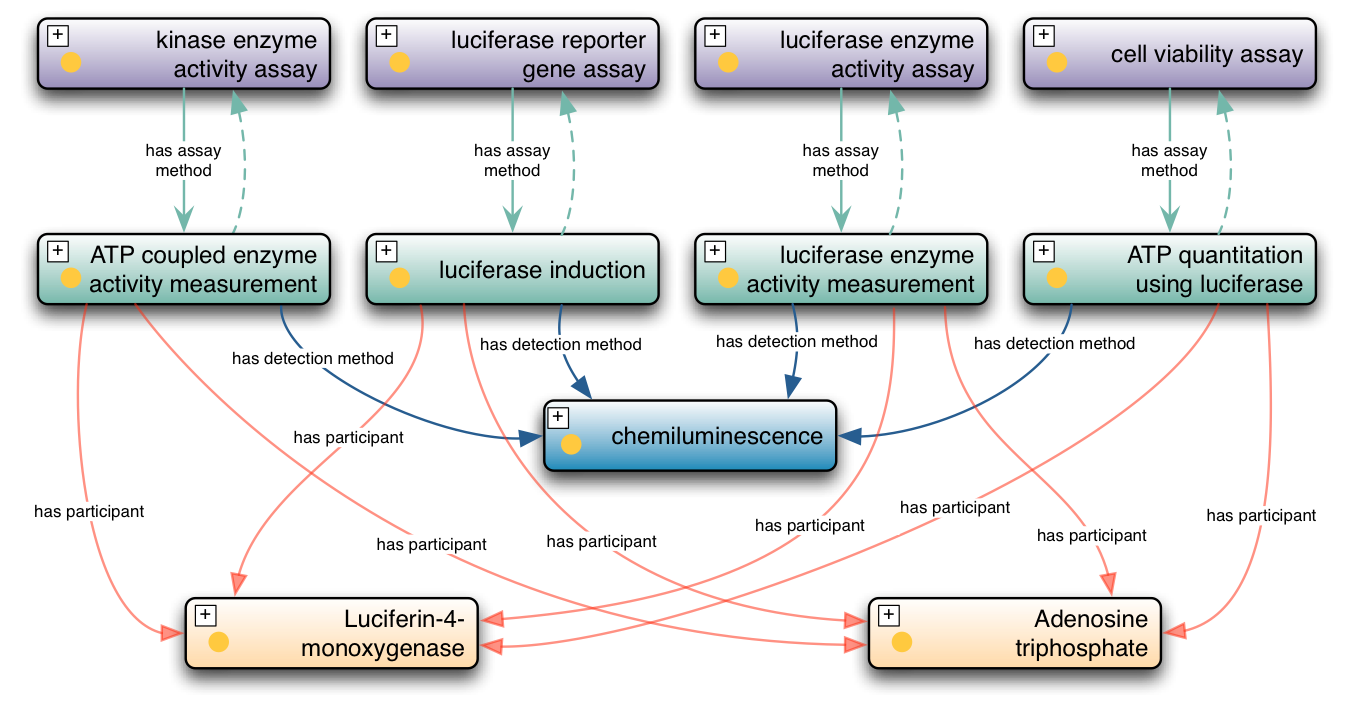
\includegraphics[width=0.9\paperwidth]{assaymodel}    
  \end{center}
\end{frame}

\begin{frame}
  \frametitle{Prior Work}
  \begin{itemize}
  \item BAO annotated datasets
    \begin{itemize}
    \item \href{http://www.ncbi.nlm.nih.gov/pubmed/24441647}{de Souza et al, 2014}; \href{http://www.ncbi.nlm.nih.gov/pubmed/23155465}{Vempati et al, 2012}
    \end{itemize}
  \item Analyzing HTS datasets using BAO
    \begin{itemize}
    \item \href{http://www.ncbi.nlm.nih.gov/pubmed/25512330}{Zander-Balderud et al, 2015}; \href{http://www.ncbi.nlm.nih.gov/pubmed/21471461}{Sch\"{u}rer et al, 2011}
    \end{itemize}
  \item Semi-automated annotation of assay descriptions using the BAO 
    \begin{itemize}
    \item \href{http://www.ncbi.nlm.nih.gov/pubmed/25165633}{Clark et al, 2014}
    \end{itemize}
  \end{itemize}
\end{frame}


\begin{frame} 
  \frametitle{Workflow}
  \begin{itemize}
  \item Extract unique BAO terms and for each term identify annotated assays
  \item Extract active compounds from this set of assays
  \item Compute fingerprint bit distribution
  \item Use these conditional bit distributions to identify the BAO terms that describe the assay that they are likely to be active in
  \end{itemize}
\end{frame}

\begin{frame}
  \frametitle{Dataset Overview}
  \begin{itemize}
  \item Extracted 4010 Pubchem AIDs from BARD
  \item Primary, confirmation, counterscreening assays
  \item 154M outcomes
  \item 740K compounds
  \item Pubchem 881-bit keys using \href{http://cdk.github.io/cdk/1.5/docs/api/org/openscience/cdk/fingerprint/PubchemFingerprinter.html}{CDK} and
    \href{https://bitbucket.org/caodac/pcfp}{NCGC} implementations  
  \item 192 unique BAO terms  
  \end{itemize}
\end{frame}

\begin{frame}
  \frametitle{Dataset Overview}
  \begin{center}
  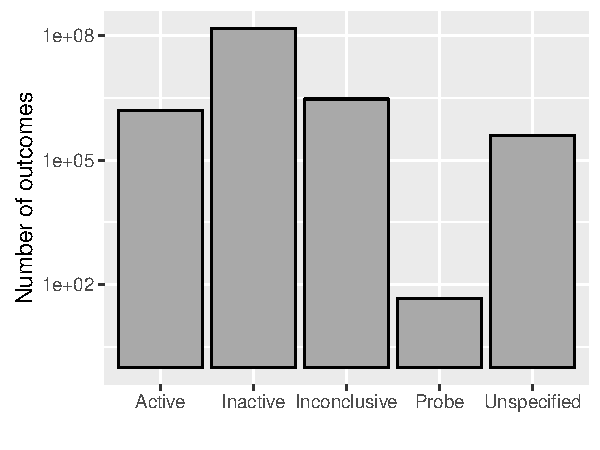
\includegraphics[width=0.5\textwidth]{img-bioassay-outcomes} 
  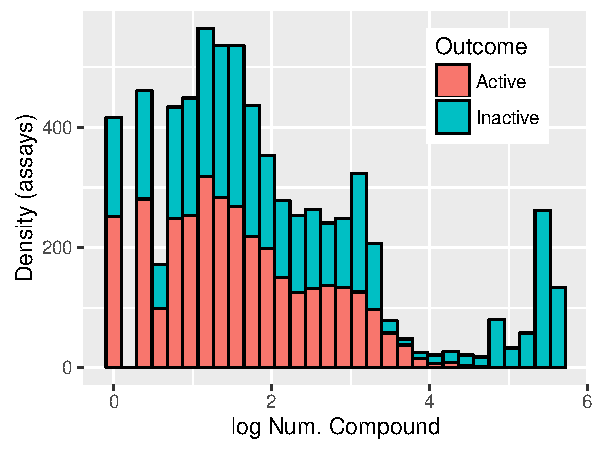
\includegraphics[width=0.5\textwidth]{img-outcomehistogram} \\
  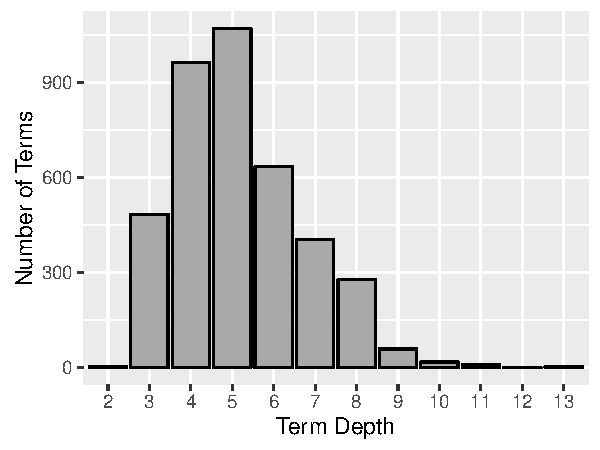
\includegraphics[width=0.5\textwidth]{img-termdepth}
  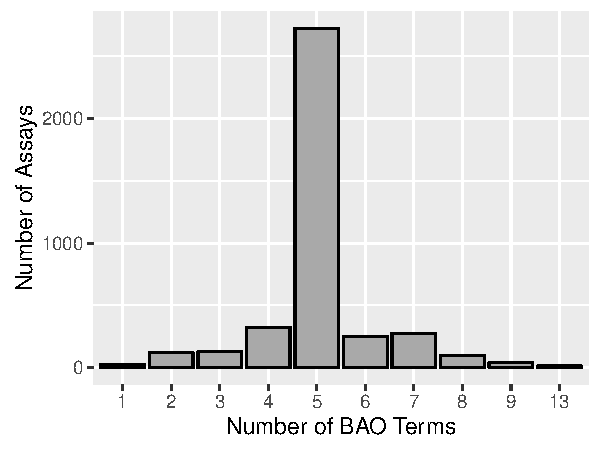
\includegraphics[width=0.5\textwidth]{img-termassaycount} \\    
  \end{center}
\end{frame}

\begin{frame}
  \frametitle{Class Imbalances}
\centering{
  \parbox{0.75\textwidth}{ Imbalanced classes are problematic, and
    some of the terms with near-balanced classes are not very specific
    (e.g., \texttt{imaging method})
  }}\vskip 1em
    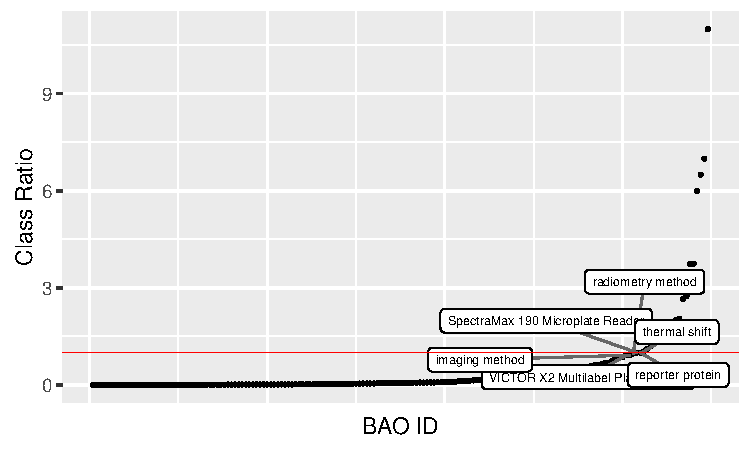
\includegraphics[width=0.9\textwidth]{img-nbclassratio-v2}
\end{frame}


%%%% per-term NB model
% \begin{frame}
%   \frametitle{Per-Term Na\"{i}ve Bayes Models}
%   \begin{itemize}
%   \item Predict liklihood of being active, given an ontology term
%     $T_i$ and given a set of  features $\{B\}$  
%   \item Model this using Na\"{i}ve Bayes in which the two classes are
%     $T_i$ and ``Other''
%   \item Results in a set of models $\{M_1, M_2, \cdots, M_N\}$ where $N$
%     is the number of unique ontology terms. \vskip 1em
%   \item For a new compound in library, obtain probability of term $T_i$ using
%     model $M_i$
%   \item Aggregate top $k$ terms from each model for each compound in
%     the library and select top $n$ terms
%   \item \textbf{Represents the set of ontology terms defining an assay in
%     which these compound would likely be active}  
%   \end{itemize}
% \end{frame}

\begin{frame}
  \frametitle{Problem formulation}
  For a given library of compounds $X$, we would like to calculate a
  ranked list \emph{relevant} $T$ of BAO terms that are most likely associated with
  $X$. Let $\mathbf{x} \in X$ and $t$ is a BAO term. The list $T$ is
  an ordered list based on the following:
  \begin{equation}
  \argmax_{i}\left\{\sum_jp(t_i|\mathbf{x}_j)\right\},
  \end{equation}
  where $p(t_i|\mathbf{x}_j)$ is the probability that BAO term $t_i$
  is associated with compound $\mathbf{x}_j$. From Bayes' rule, we have
  \[
    p(t_i|\mathbf{x}_j) = \frac{p(\mathbf{x}_j|t_i)p(t_i)}{p(\mathbf{x}_j)}
    \quad\hbox{or} \quad p(t_i|\mathbf{x}_j) \propto p(\mathbf{x}_j|t_i)p(t_i).
  \]
  Given that BAO terms are annotated at the assay level, we instead
  have 
  \begin{equation}
    p(t_i|\mathbf{x}_j) \propto p(t_i)\sum_kp(\mathbf{x}_j|a_k)p(a_k|t_i),
  \end{equation}
  where $a_k$ is a BAO annotated assay.
\end{frame}

\begin{frame}
  \frametitle{A Bayesian Approach for Ranking}
  Note that $p(\mathbf{x}_j|a_k)$ is the sampling function specified
  over only \emph{active} compounds in assay $a_k$. In our model,
  $\mathbf{x}_j$ is defined as independent Bernoulli distribution with
  parameter $\theta$, i.e., 
\[ p(\mathbf{x}_j|a_k) =
\prod_i\theta_i^{x_{ji}}(1-\theta_i)^{1-x_{ji}},\]
where $x_{ji}\in\{0,1\}$ is the $i$-th bit of the PubChem
substructural fingerprint. 

\begin{block}{}
\begin{color}{blue}
Learning BAO terms for a library of
compounds amounts to estimating $\theta$, $p(t_i)$, and $p(a_k|t_i)$. 
\end{color}
\end{block}
\end{frame}

% \begin{frame}
%   \frametitle{Per-Term Na\"{i}ve Bayes Models}
%   \begin{itemize}
%   \item Predict liklihood of ontology term $T_i$ given a set of  features $\{B\}$  
%   \item Model this using Na\"{i}ve Bayes where we compute XXX
%   \item Results in two set of models $\{M_1, M_2, \cdots, M_N\}$, for
%     actives and inactives where $N$ is the number of unique ontology
%     terms. \vskip 1em
%   \item For a new compound in library, obtain probability of term $T_i$ using
%     model $M_i$ for actives, XXX
%   \item Aggregate top $k$ terms from each model for each compound in
%     the library and select top $n$ terms
%   \item \textbf{Represents the set of ontology terms defining an assay in
%     which these compound would likely be active}  
%   \end{itemize}
% \end{frame}

\begin{frame}
  \frametitle{Per-Term Activity Classifier}
  \begin{itemize}
  \item For a given ontology term $T_i$, predict whether a compound
    will be active or not 
  \item Model this using Na\"{i}ve Bayes, where we extract set of
    actives and inactives from assays annotated with $T_i$
  \item Results in a set of models $\{M_1, M_2, \cdots, M_N\}$,
 \vskip 1em
  \item For a new compound in library, obtain probability of being
    active for term $T_i$ for all $i$ and take top $k$ terms
  \item Aggregate top $k$ terms from all compounds in library
  \item \textbf{Represents the set of ontology terms defining an assay in
    which these compounds would likely be active}  
  \end{itemize}
\end{frame}


% \begin{frame}
%   \frametitle{Training Set Performance}
%   \begin{itemize}
%   \item Matthews Correlation Coefficient
%   \end{itemize}
% \end{frame}


\begin{frame}
  \frametitle{Test Libraries}
  \begin{itemize}
  \item Considered several libraries to test out the approach
  \item MIPE (1912 compounds) - Approved, investigational drugs, constructed for functional diversity
  \item LOPAC (1280 compounds) - Diverse library, designed for enrichment of bioactivity
  \item Natural Products (5000 compounds)
  \item 1000 member subset of ChEMBL GPCR collection 
  \item 1000 member subset of ChEMBL Kinase collection
  \end{itemize}
\end{frame}

\begin{frame}
  \frametitle{Test Libraries}
In the Pubchem fingerprint space, the libraries are not very different
\vskip 1em
  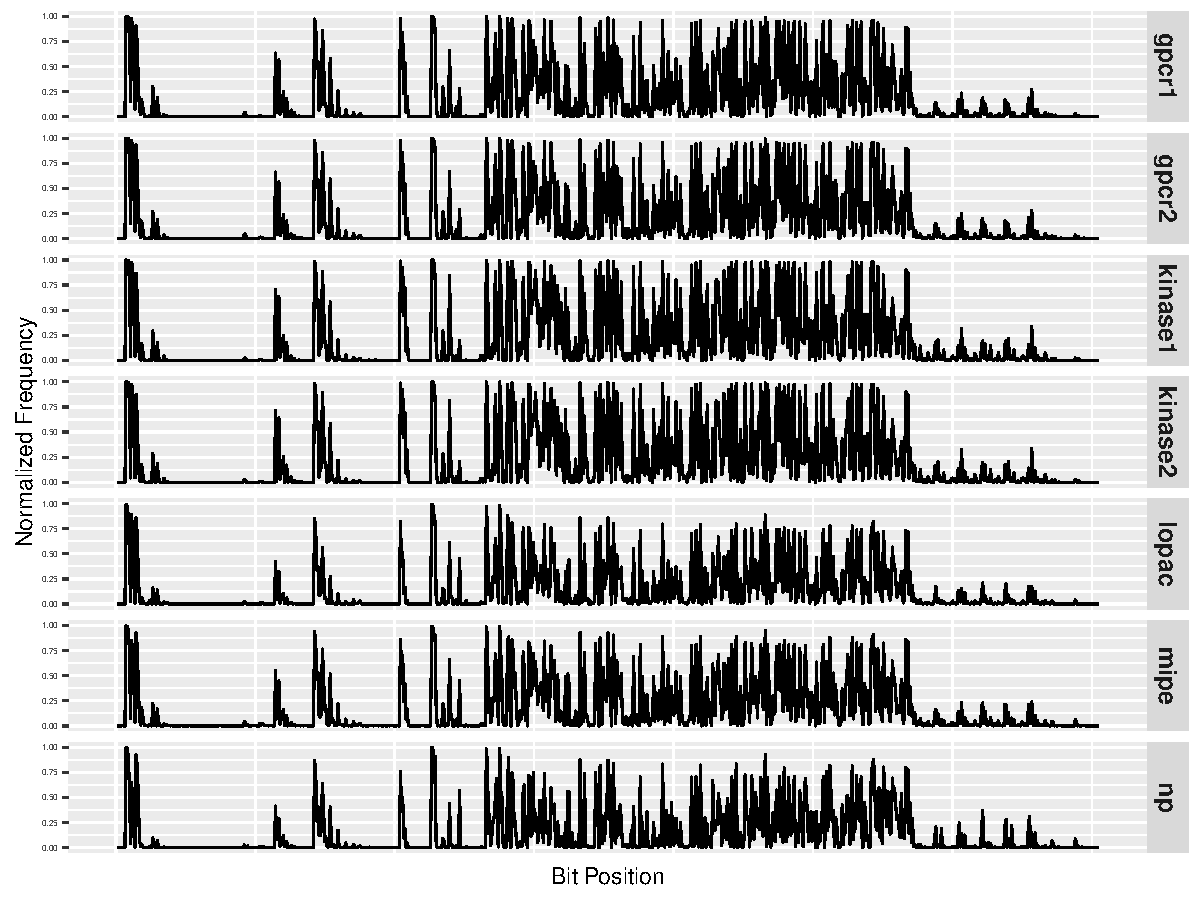
\includegraphics[width=0.9\textwidth]{img-psetbs.pdf}  
\end{frame}

\begin{frame}
  \frametitle{Test Libraries - Distance Matrix}
  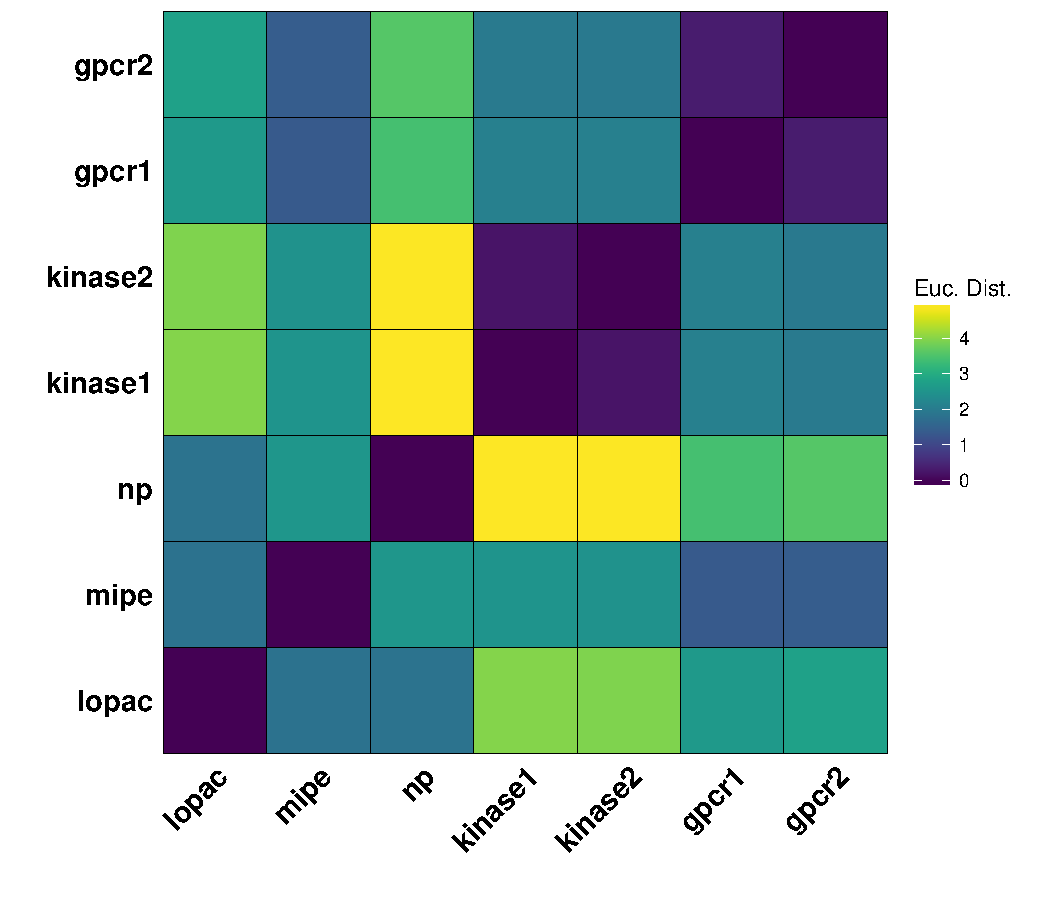
\includegraphics[width=0.9\textwidth]{img-psetbs-distmap.pdf}  
\end{frame}

\begin{frame}
  \frametitle{Prediction Workflow}
  \begin{columns}[t]
    \begin{column}{0.5\textwidth}
      \textbf{Bayesian Ranking}
      \begin{itemize}
      \item Compute liklihood of all terms for each compound
      \item Aggregate across library (mean liklihood) and take top $k$
      \end{itemize}
    \end{column}
    \begin{column}{0.5\textwidth}
      \textbf{Activity Models}
      \begin{itemize}
      \item For molecules predicted active, collect corresponding terms
      \item Retain the top $k$ most frequent terms across the library
      \end{itemize}
    \end{column}
  \end{columns}
\vskip 2em
  \centering{
    \parbox{0.75\textwidth}{\textbf{We take the top $k$  terms as
      the set of annotations describing an assay in which the library
      will show activity in}}
  }
\end{frame}


\begin{frame}
  \frametitle{Result - Bayesian Ranking}
  \begin{center}
    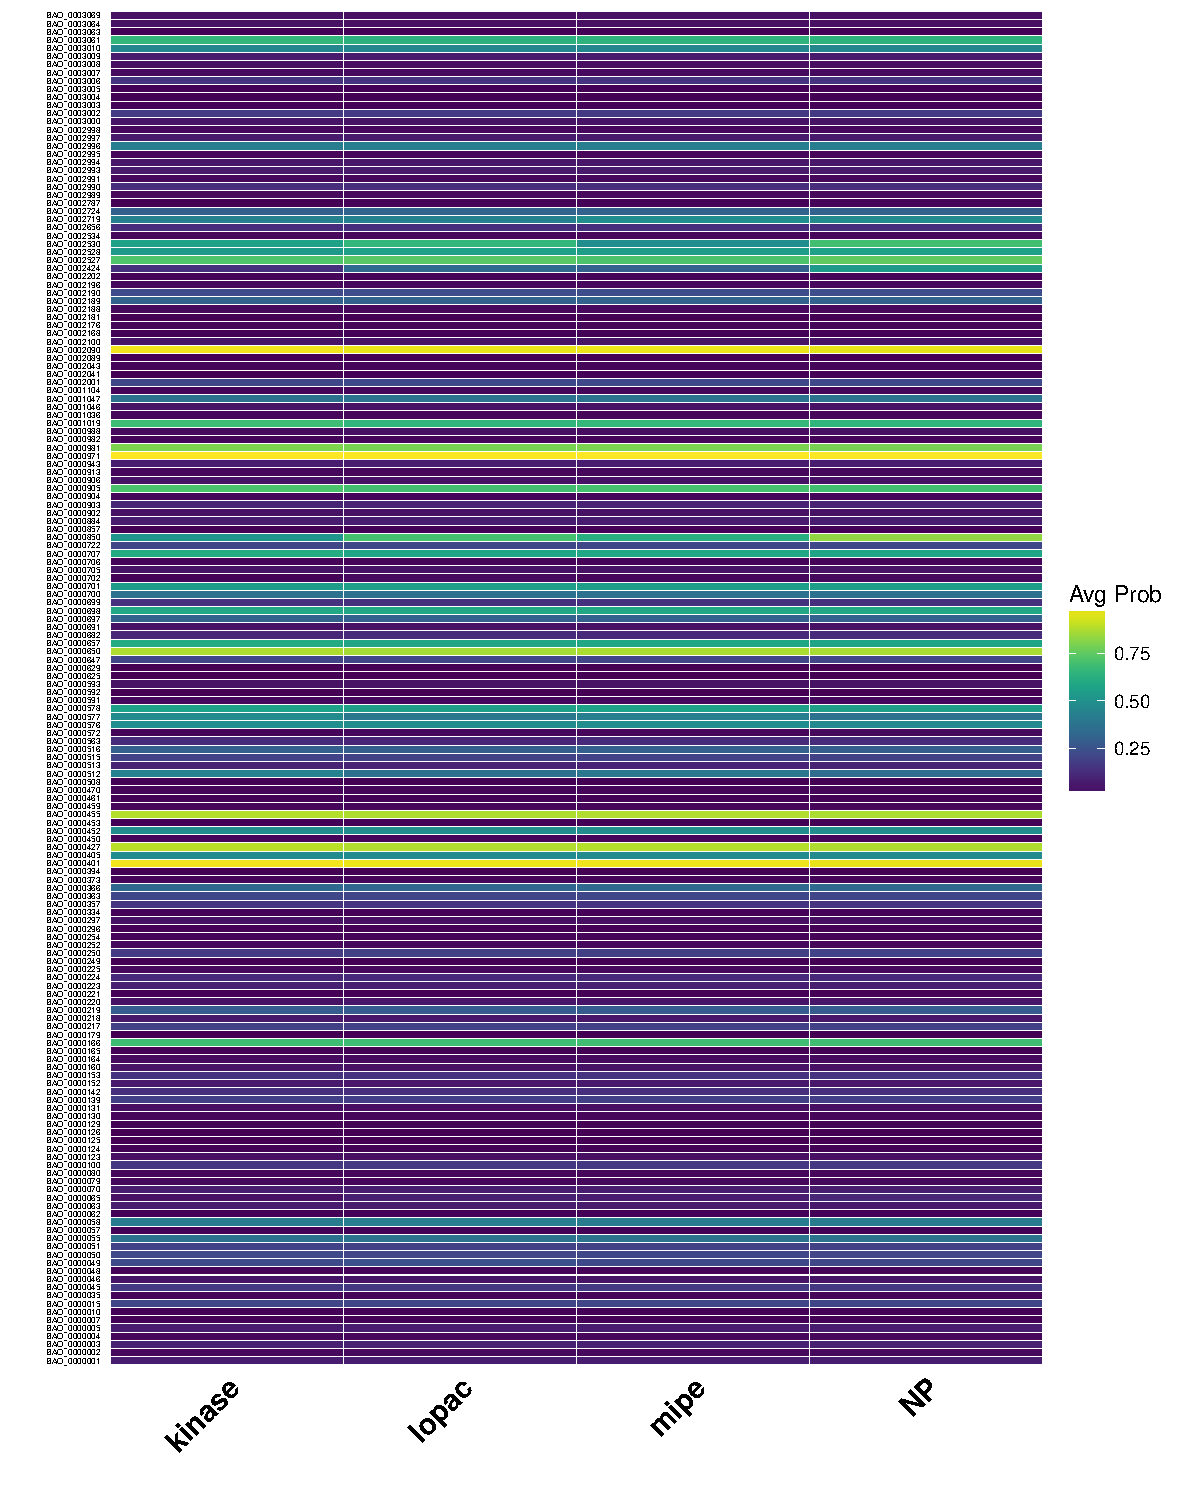
\includegraphics[height=0.9\textheight]{img-predset-rankedterms-trung.pdf}      
  \end{center}
\end{frame}

  \begin{frame}
    \frametitle{Result - Per Term Activity Classifier}
    \begin{center}
      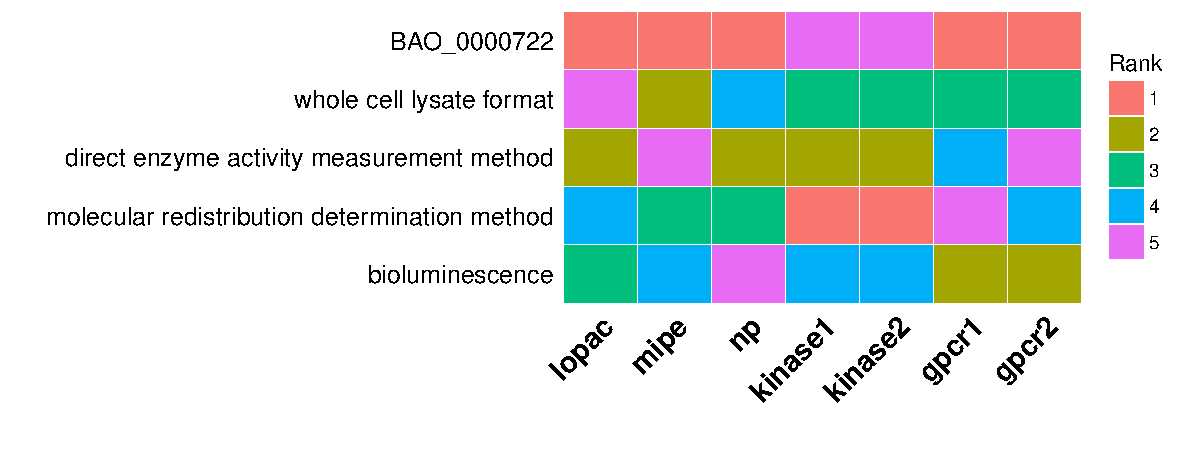
\includegraphics[width=1.1\textwidth]{img-predset-rankedterms.pdf}      
    \end{center}
  \end{frame}

  \begin{frame}
    \frametitle{What's Different Between Libraries?}
      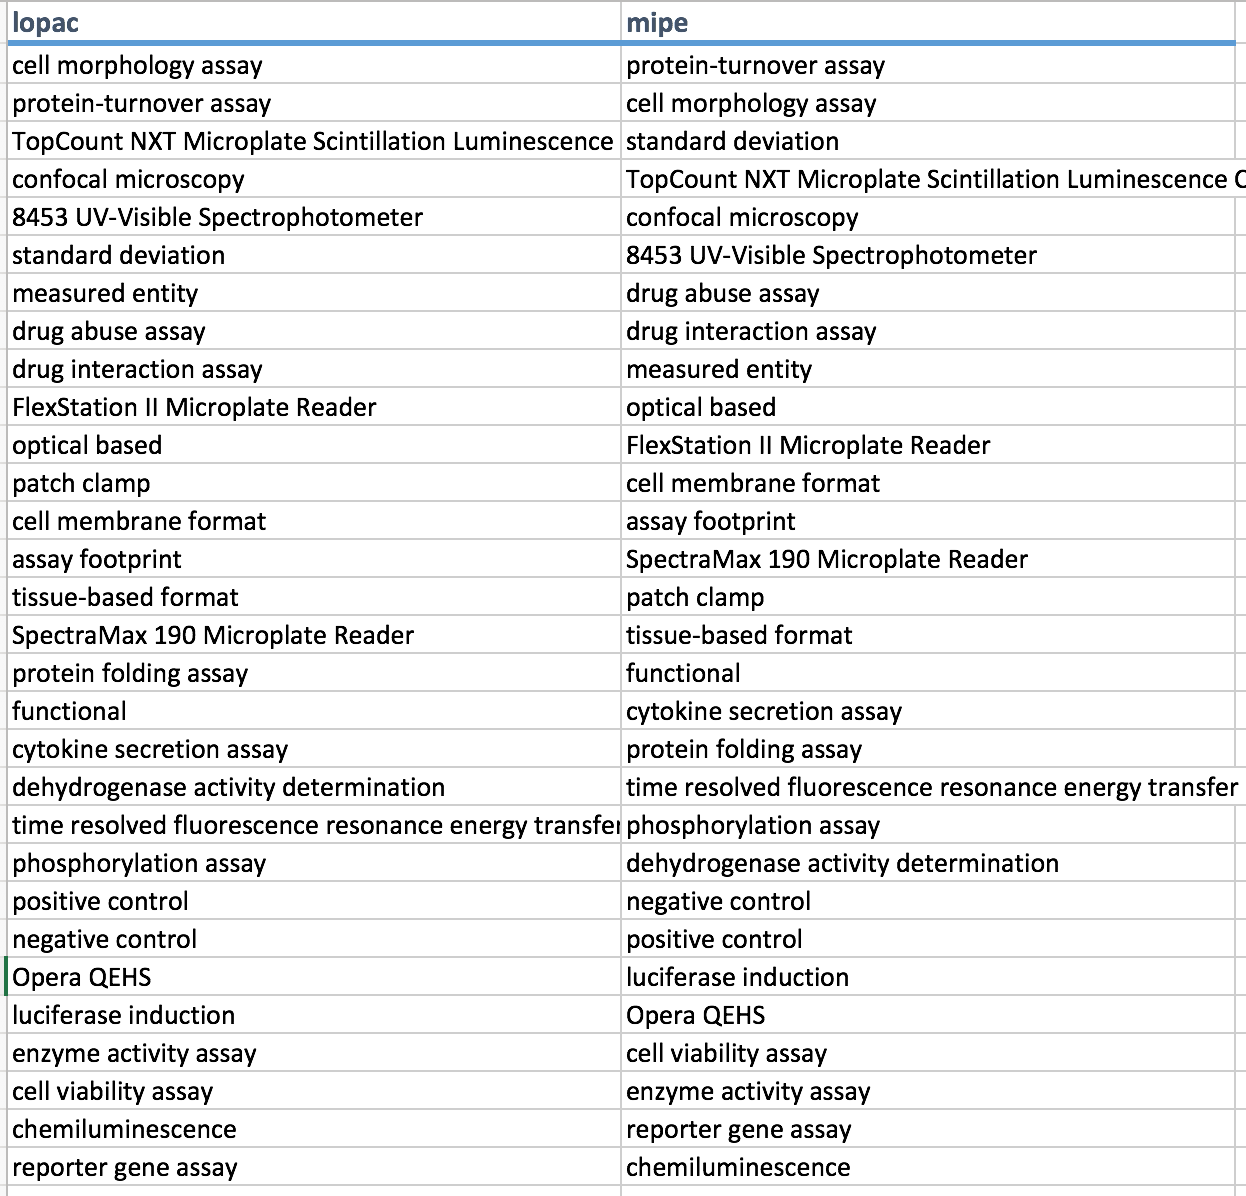
\includegraphics[height=0.9\textheight]{img-diff-lopac-vs-mipe}      
  \end{frame}
  \begin{frame}
    \frametitle{What's Different Between Libraries?}
      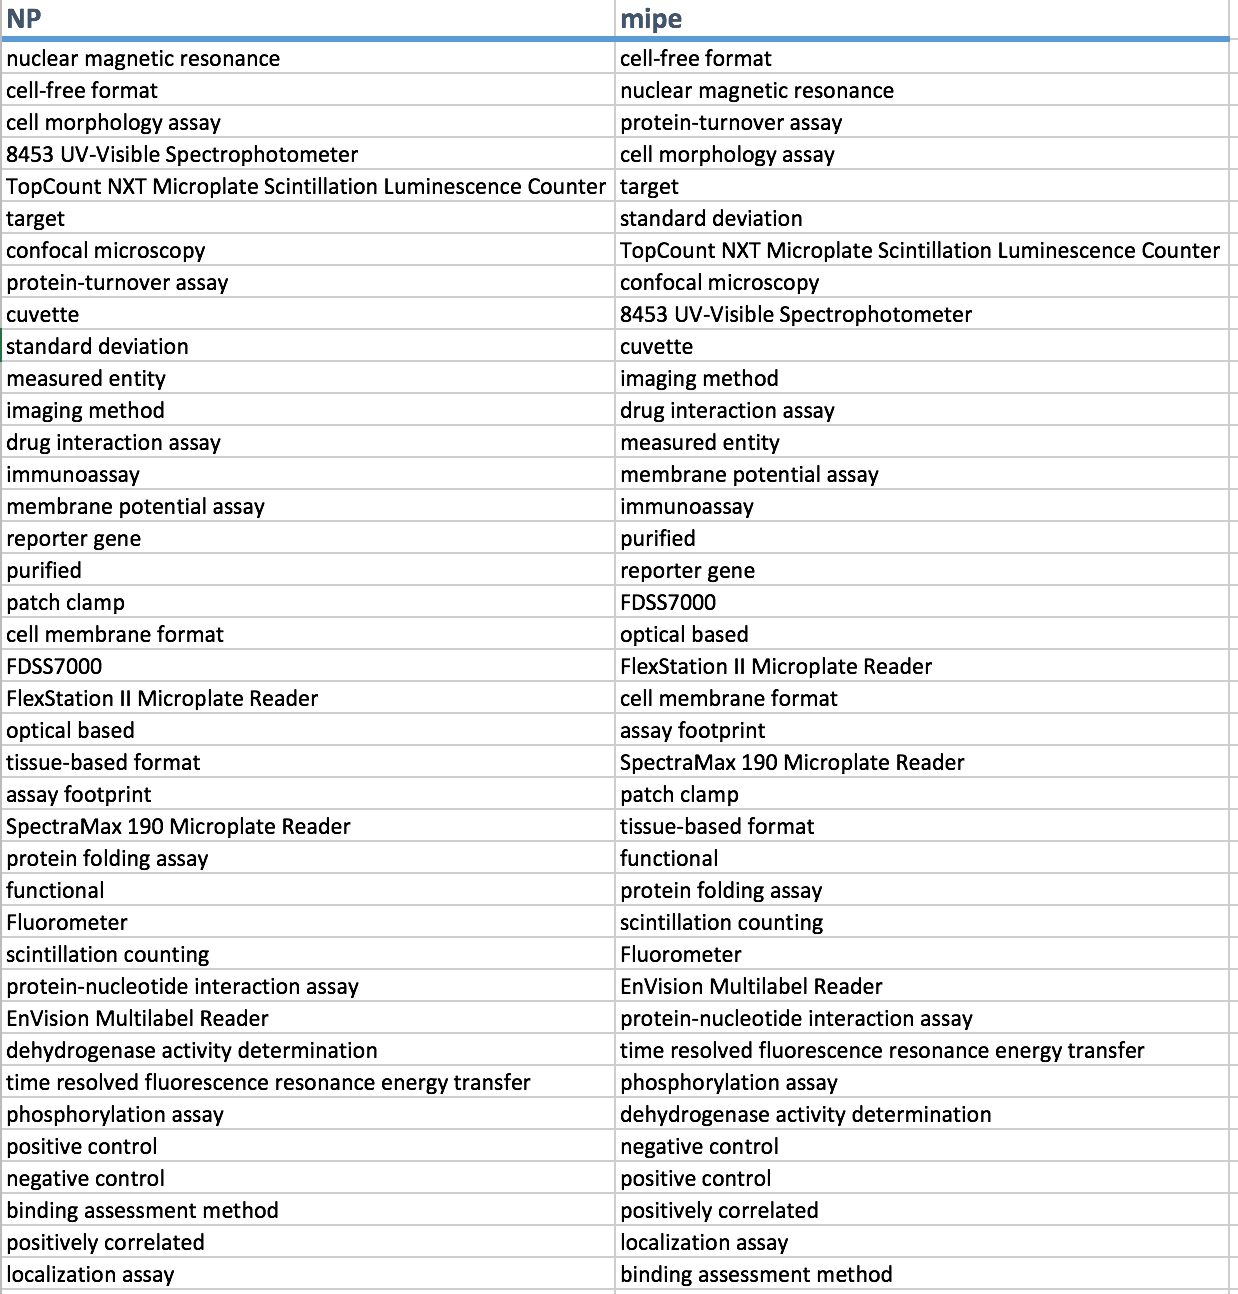
\includegraphics[height=0.9\textheight]{img-diff-np-vs-mipe}      
  \end{frame}

\begin{frame}
  \frametitle{Term Depth vs Rank}
  \begin{itemize}
  \item Do more specific terms get ranked highly?
  \item Which terms get ranked is driven by frequency of usage across assays
  \end{itemize}
\end{frame}

%%%% Ending slides
\begin{frame}
  \frametitle{Pitfalls}
  \centering{
    \parbox{0.75\textwidth}{
      \textit{\color{red}If sufficiently annotated, compound behavior can be 
        correlated to assay and biology characteristics}}
}
\vskip 1em
  \begin{itemize}
  \item A very abstract, possibly lossy, view of the effect of compounds on biology
  \item Depends on correct and meaningful annotations
  \item Annotations terms are context dependent, but this may not be considered when annotating a dataset
  \item BAO terms exhibit hierarchical relationships and ignoring them
    is simplistic
  \end{itemize}
\vskip 2em
\Large{\href{https://spotlite.nih.gov/ncats/acs-fall-2016/tree/master}{Source
code and slides}}
\end{frame}

\begin{frame}
  \frametitle{Acknowledgements}
  \begin{itemize}
  \item Qiong Cheng (U. Miami)
  \item Stephan Sch\"{u}rer (U. Miami)  
  \end{itemize}
\end{frame}
\end{document}
